\documentclass[12pt, a4paper]{article}
\usepackage[utf8]{inputenc}
\usepackage{graphicx}
\usepackage{amsmath}
\usepackage{booktabs}
\usepackage{geometry}
\usepackage{hyperref}
\usepackage{setspace}

% 设置页面边距和行距
\geometry{a4paper, margin=1in}
\setstretch{1.15}

\title{\textbf{Predicting Heart Failure Mortality: A Comparative Analysis of Machine Learning and Deep Learning Models}}
\author{Haoyu Wang}
\date{March 2026}

\begin{document}

\maketitle

\begin{abstract}
Predicting heart failure mortality is critical for proactive clinical decision-making and patient management. This study conducts a comparative analysis between a traditional statistical model, Logistic Regression, and a deep learning approach, represented by a Multi-Layer Perceptron (MLP) classifier. Utilizing a clinical dataset of 299 patients, we evaluated the models based on accuracy and Area Under the ROC Curve (AUC). Our findings indicate that Logistic Regression achieved a superior accuracy of 81.7\% (AUC=0.859), outperforming the MLP model (accuracy 75.0\%, AUC=0.746). Feature importance analysis further revealed that serum creatinine and ejection fraction are the most critical predictors of mortality. The study concludes that for small-scale clinical datasets, traditional linear models offer better robustness and interpretability without the risk of overfitting associated with complex neural networks.
\end{abstract}

\section{Introduction}
Heart failure is a complex clinical syndrome and a leading cause of mortality worldwide. Early and accurate prediction of survival can significantly enhance personalized treatment plans and resource allocation in intensive care units \cite{chicco2020}. Recently, machine learning (ML) and artificial intelligence (AI) have demonstrated immense potential in extracting prognostic patterns from electronic health records (EHR) and clinical datasets \cite{obermeyer2016}. 

However, the application of deep learning algorithms in the medical domain often faces challenges related to data scarcity and model interpretability \cite{rajkomar2018}. This study aims to bridge this gap by systematically comparing the predictive performance of a standard Multi-Layer Perceptron (MLP) neural network against traditional Logistic Regression on a specialized heart failure dataset.

\section{Methodology}

\subsection{Data Preprocessing}
The study utilized a clinical dataset comprising 299 patient records with 13 features. To ensure data integrity and reproducibility, we implemented median imputation to address any missing values. The dataset was partitioned using \textbf{Stratified Sampling} (80\% training, 20\% testing) to maintain the original class distribution of mortality events. Given the sensitivity of distance-based and gradient-descent algorithms to feature scales, all numerical features were standardized using Z-score scaling.

\subsection{Exploratory Analysis and Proposed Workflow}
Prior to model training, exploratory data analysis was conducted to understand the underlying clinical relationships. Figure \ref{fig:heatmap} displays the correlation heatmap of the clinical variables, highlighting potential multicollinearity and preliminary associations with the target variable. 

\begin{figure}[htbp]
    \centering
    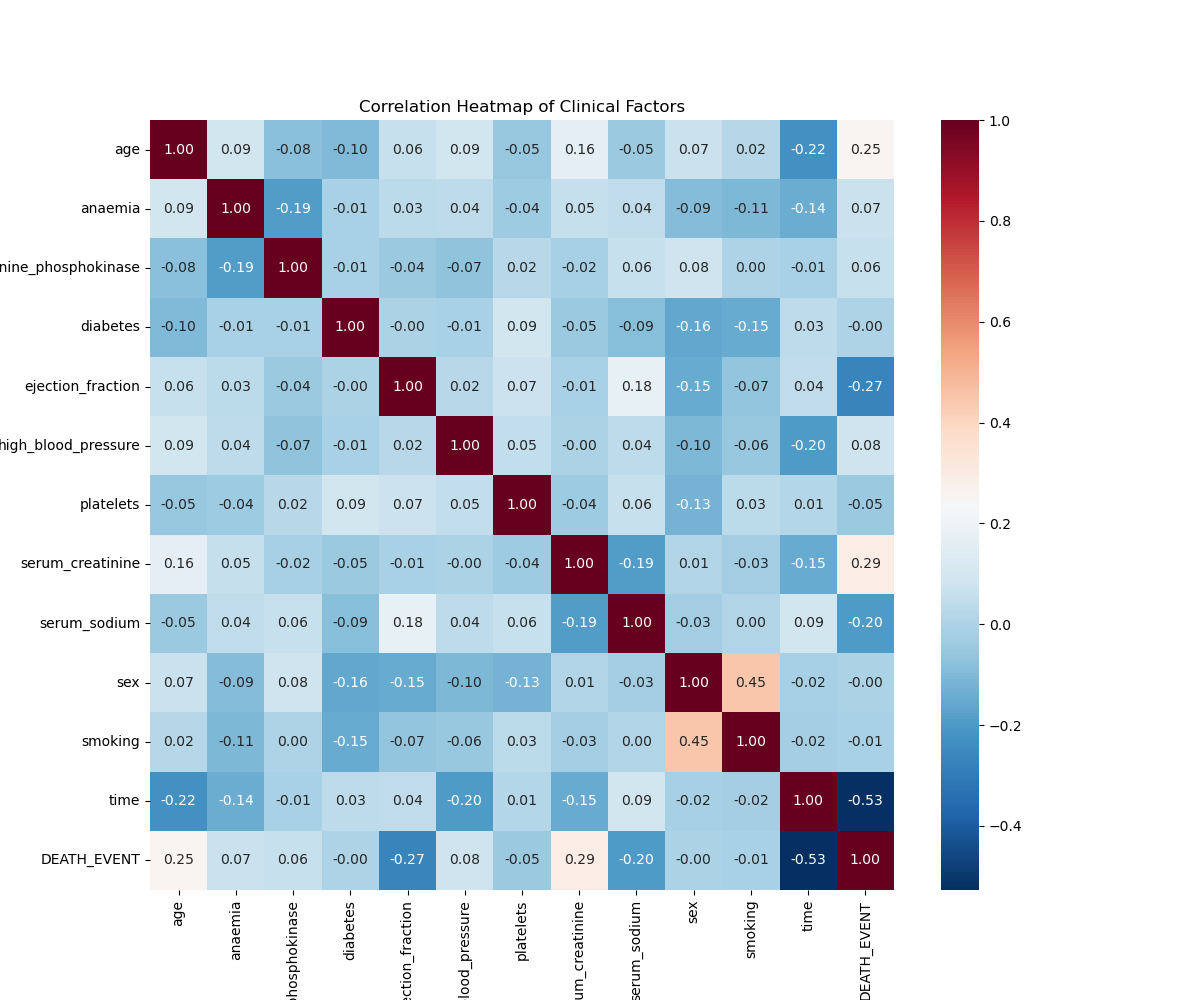
\includegraphics[width=0.7\textwidth]{correlation_heatmap.png}
    \caption{Correlation heatmap of clinical features, demonstrating variable interactions.}
    \label{fig:heatmap}
\end{figure}

The overall experimental methodology follows a structured pipeline, from data ingestion to model deployment, as illustrated in the AI workflow diagram (Figure \ref{fig:workflow}).

\begin{figure}[htbp]
    \centering
    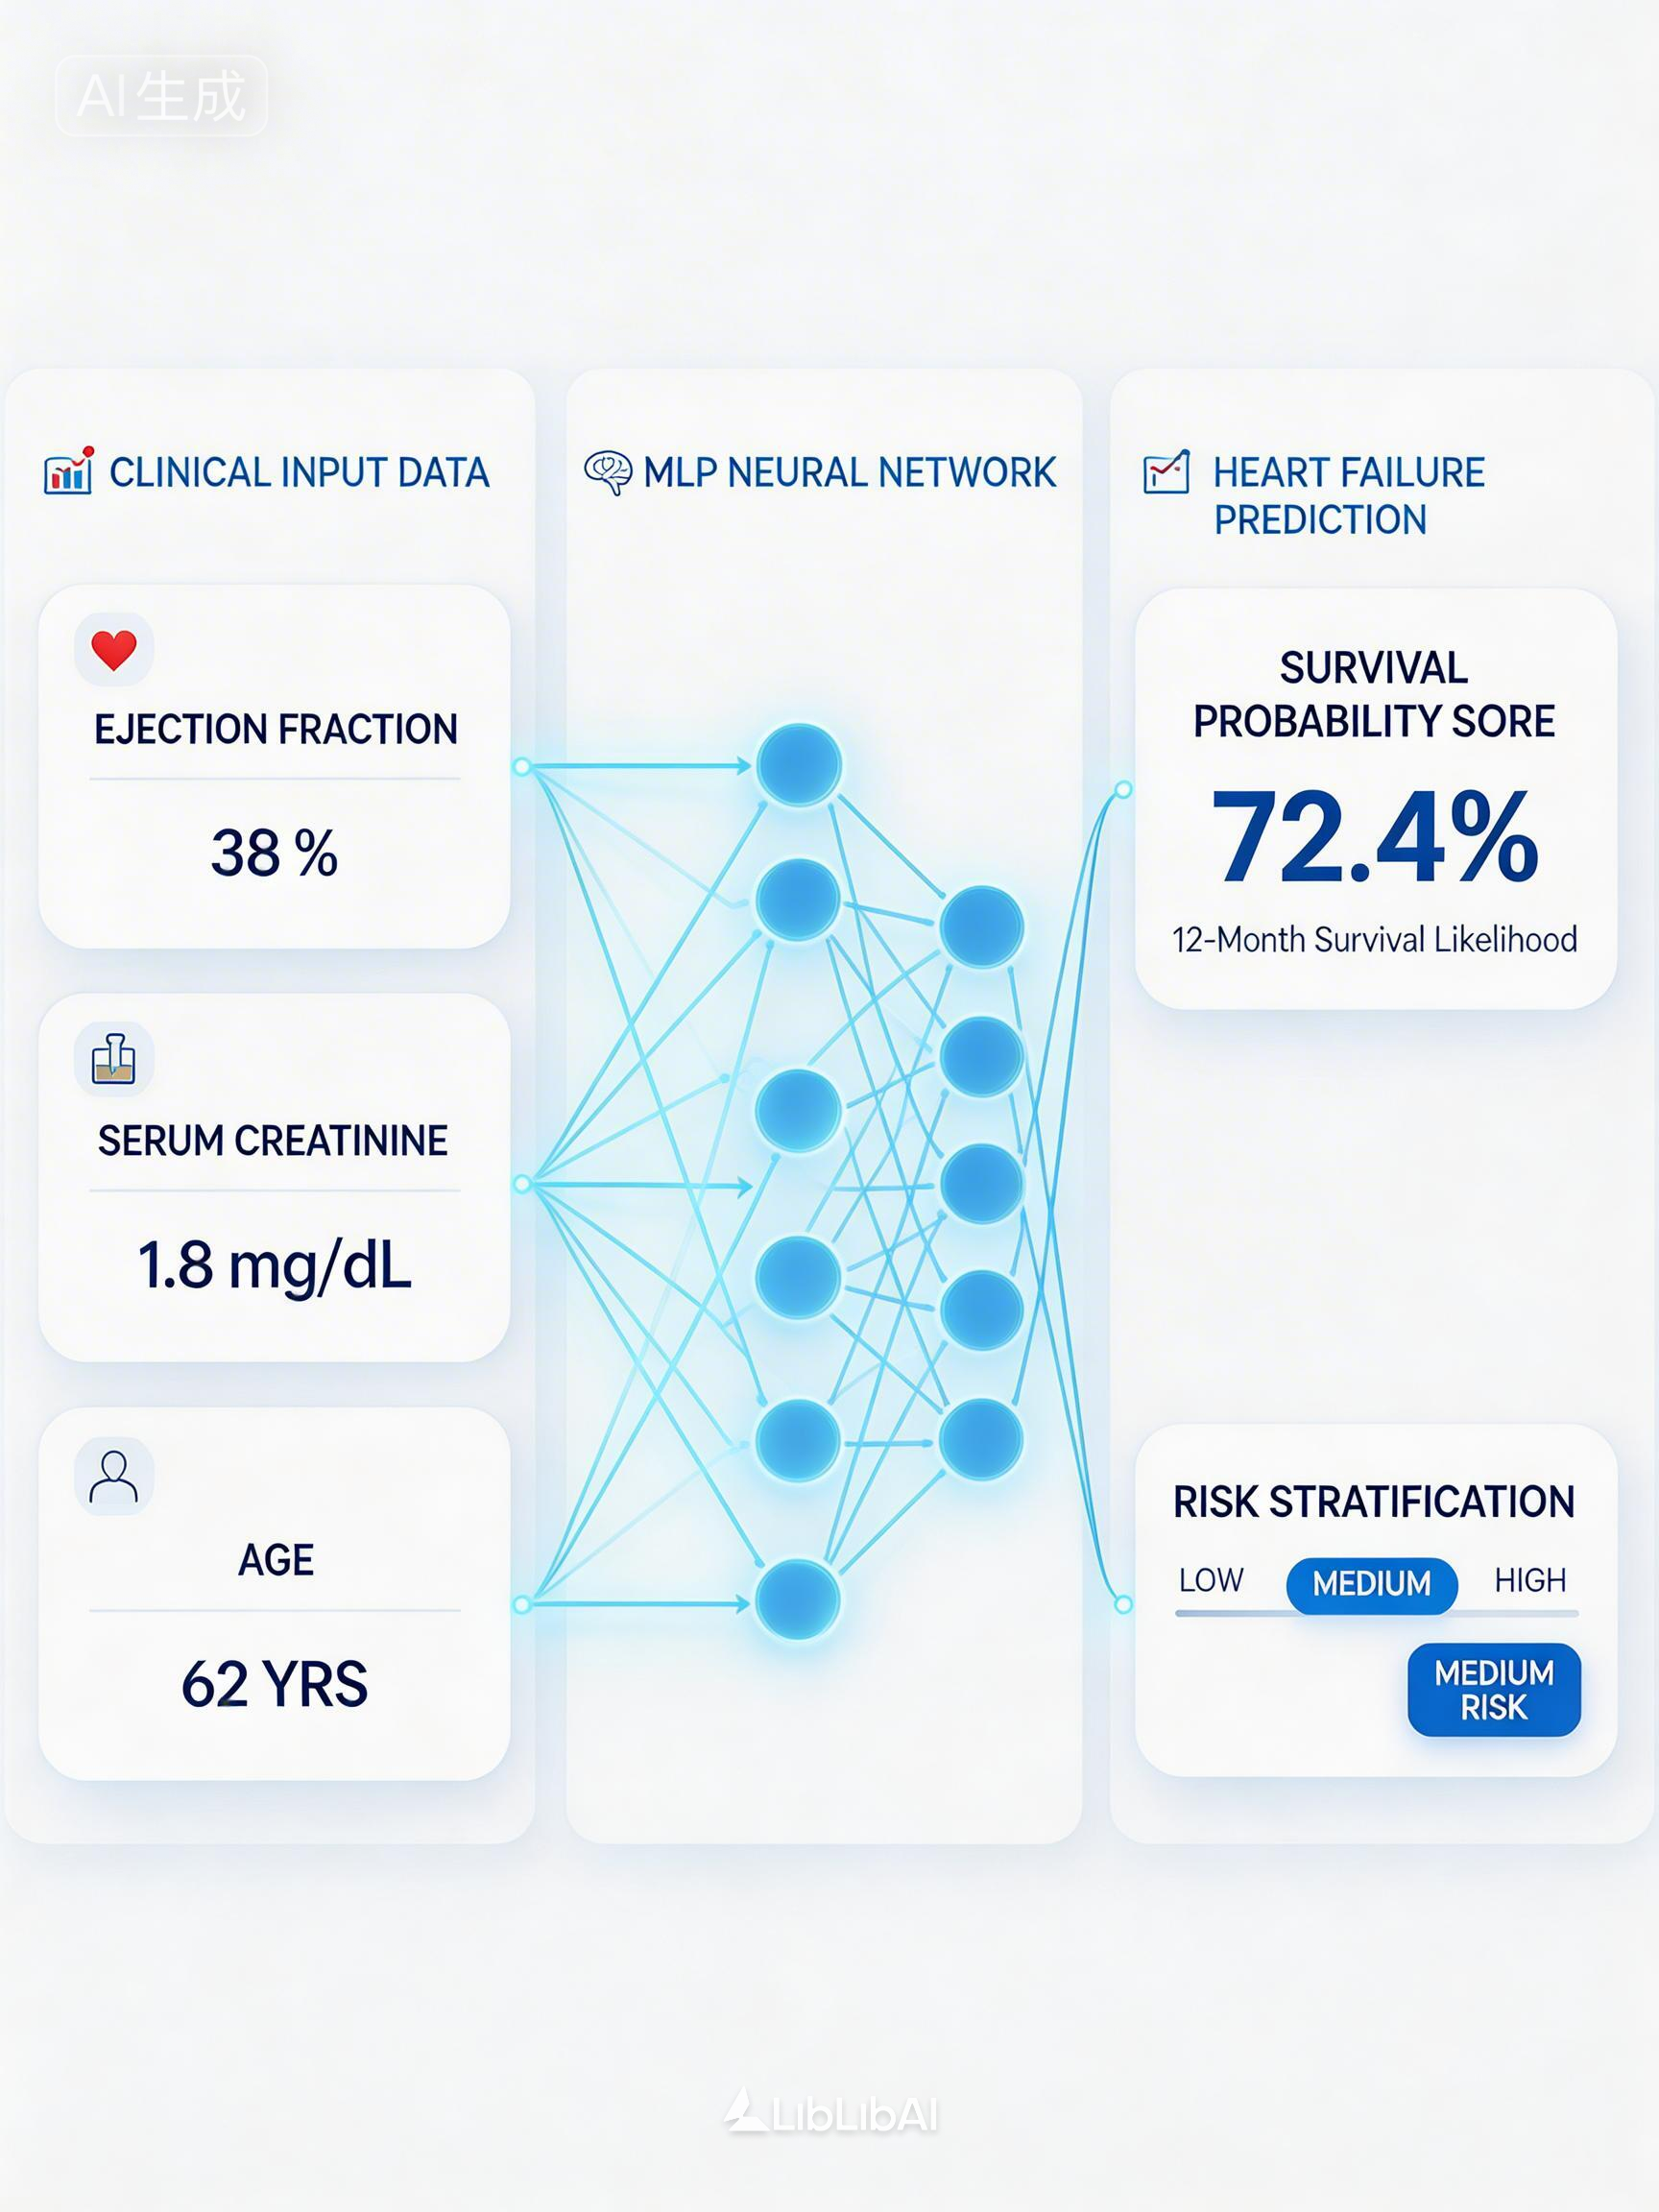
\includegraphics[width=0.7\textwidth]{ai_workflow.jpg}
    \caption{Proposed AI workflow for heart failure prediction and clinical integration.}
    \label{fig:workflow}
\end{figure}

\section{Results}

\subsection{Feature Importance Analysis}
Understanding which clinical indicators drive the prediction is essential for medical trust. A Random Forest feature importance analysis was conducted (Figure \ref{fig:importance}). The results identified \textbf{Serum Creatinine} and \textbf{Ejection Fraction} as the most critical predictors of patient mortality. This aligns with existing physiological knowledge, as these metrics directly reflect renal function and cardiac pumping efficiency, respectively \cite{ahmad2017}.

\begin{figure}[htbp]
    \centering
    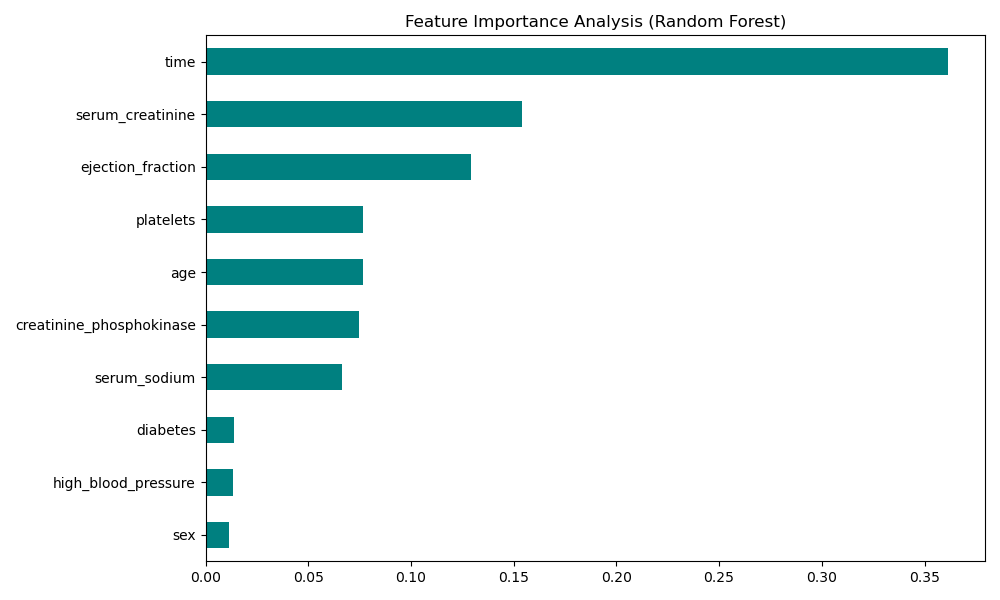
\includegraphics[width=0.7\textwidth]{feature_importance.png}
    \caption{Clinical features ranked by Random Forest importance criteria.}
    \label{fig:importance}
\end{figure}

\subsection{Model Performance and Evaluation}
The quantitative comparison between the models is detailed in Table \ref{tab:performance}. Logistic Regression demonstrated a higher overall accuracy (0.817) compared to the MLP Classifier (0.750). 

\begin{table}[htbp]
\centering
\caption{Model Performance Comparison on Test Set}
\label{tab:performance}
\begin{tabular}{lcc}
\toprule
\textbf{Model} & \textbf{Accuracy} & \textbf{AUC} \\ 
\midrule
Logistic Regression & 0.817 & 0.859 \\ 
MLP Classifier & 0.750 & 0.746 \\ 
\bottomrule
\end{tabular}
\end{table}

To further evaluate the discriminative ability of the classifiers across different thresholds, Receiver Operating Characteristic (ROC) curves were plotted (Figure \ref{fig:roc}). The Logistic Regression model achieved a significantly higher Area Under the Curve (AUC = 0.859), indicating superior sensitivity and specificity balance.

\begin{figure}[htbp]
    \centering
    
\includegraphics[width=0.65\textwidth]{roc_curve.png}
    \caption{ROC curves comparing the predictive capability of Logistic Regression and MLP.}
    \label{fig:roc}
\end{figure}

\section{Discussion and Conclusion}
The empirical results suggest that the superior performance of Logistic Regression is primarily due to the limited sample size (N=299). Deep learning models like MLP require vast amounts of data to optimize their complex weight matrices effectively; otherwise, they are highly susceptible to overfitting the training distribution \cite{rajkomar2018}. Conversely, simpler linear models impose a strong inductive bias that remains robust even with sparse clinical data. 

In conclusion, while deep learning holds promise for large-scale medical imaging and genomics, traditional statistical machine learning models remain the optimal choice for small-to-medium tabular clinical datasets in terms of both performance and interpretability.

\begin{thebibliography}{99}

\bibitem{chicco2020} 
Chicco, D., \& Jurman, G. (2020). Machine learning can predict survival of patients with heart failure from serum creatinine and ejection fraction alone. \textit{BMC Medical Informatics and Decision Making}, 20(1), 16.

\bibitem{obermeyer2016} 
Obermeyer, Z., \& Emanuel, E. J. (2016). Predicting the future—big data, machine learning, and clinical medicine. \textit{The New England Journal of Medicine}, 375(13), 1216.

\bibitem{rajkomar2018} 
Rajkomar, A., Dean, J., \& Kohane, I. (2018). Machine learning in medicine. \textit{The New England Journal of Medicine}, 380(14), 1347-1358.

\bibitem{ahmad2017}
Ahmad, T., Munir, A., Bhatti, S. H., Aftab, M., \& Raza, M. A. (2017). Survival analysis of heart failure patients: A case study. \textit{PLOS One}, 12(7), e0181001.

\end{thebibliography}

\end{document}